\documentclass[twoside]{article}
\setlength{\oddsidemargin}{0.25 in}
\setlength{\evensidemargin}{-0.25 in}
\setlength{\topmargin}{-0.6 in}
\setlength{\textwidth}{6.5 in}
\setlength{\textheight}{8.5 in}
\setlength{\headsep}{0.75 in}
\setlength{\parindent}{0 in}
\setlength{\parskip}{0.1 in}

%
% ADD PACKAGES here:
%

\usepackage{amsmath,amsfonts,graphicx, booktabs, array, float}

%
% The following commands set up the lecnum (lecture number)
% counter and make various numbering schemes work relative
% to the lecture number.
%
\newcounter{lecnum}
\renewcommand{\thepage}{\arabic{page}}
\renewcommand{\thesection}{\arabic{section}}
\renewcommand{\theequation}{\arabic{equation}}
\renewcommand{\thefigure}{\arabic{figure}}
\renewcommand{\thetable}{\arabic{table}}
\renewcommand{\listfigurename}
{Code and Outputs}

% The following macro is used to generate the header.
%
\newcommand{\lecture}[4]{
   \pagestyle{myheadings}
   \thispagestyle{plain}
   \newpage
   \setcounter{lecnum}{#1}
   \setcounter{page}{1}
   \noindent
   \begin{center}
   \framebox{
      \vbox{\vspace{2mm}
    \hbox to 6.28in { {\bf Math 5610/6860: Introduction to Numerical Analysis I \hfill Fall 2023} }
       \vspace{4mm}
       \hbox to 6.28in { {\Large \hfill Project: #2  \hfill} }
       \vspace{2mm}
       \hbox to 6.28in { {\it Instructor: #3 \hfill Name: #4} }
      \vspace{2mm}}
   }
   \end{center}
   \markboth{Project: #2}{Project: #2}

 %  {\bf Note}: {\it LaTeX template courtesy of UC Berkeley EECS dept.}

 %  {\bf Disclaimer}: {\it These notes have not been subjected to the
 %  usual scrutiny reserved for formal publications. They may be
 %  distributed outside this class only with the permission of the
%   Instructor.} \vspace*{4mm}
}
%
% Convention for citations is authors' initials followed by the year.
% For example, to cite a paper by Leighton and Maggs you would type
% \cite{LM89}, and to cite a paper by Strassen you would type \cite{S69}.
% (To avoid bibliography problems, for now we redefine the \cite command.)
% Also commands that create a suitable format for the reference list.
\renewcommand{\cite}[1]{[#1]}
\def\beginrefs{\begin{list}%
        {[\arabic{equation}]}{\usecounter{equation}
         \setlength{\leftmargin}{2.0truecm}\setlength{\labelsep}{0.4truecm}%
         \setlength{\labelwidth}{1.6truecm}}}
\def\endrefs{\end{list}}
\def\bibentry#1{\item[\hbox{[#1]}]}

%Use this command for a figure; it puts a figure in wherever you want it.
%usage: \fig{NUMBER}{SPACE-IN-INCHES}{CAPTION}
\newcommand{\fig}[3]{
			\vspace{#2}
			\begin{center}
			Figure \thelecnum.#1:~#3
			\end{center}
	}
% Use these for theorems, lemmas, proofs, etc.
\newtheorem{theorem}{Theorem}[lecnum]
\newtheorem{lemma}[theorem]{Lemma}
\newtheorem{proposition}[theorem]{Proposition}
\newtheorem{claim}[theorem]{Claim}
\newtheorem{corollary}[theorem]{Corollary}
\newtheorem{definition}[theorem]{Definition}
\newenvironment{proof}{{\bf Proof:}}{\hfill\rule{2mm}{2mm}}

% **** IF YOU WANT TO DEFINE ADDITIONAL MACROS FOR YOURSELF, PUT THEM HERE:

% syntax:
% \newcommand\NAME[ARG_COUNT]{expr #1 #2 ... etc}
\newcommand\name{Cobi Toeun (u1230512)}
\newcommand\E{\mathbb{E}}
\newcommand\R{\mathbb{R}}
\newcommand\D{\mathscr{D}}
\newcommand\Loss{\mathscr{L}}

% usage: \colvec {3}{a}{b}{c}
\newcount\colveccount
\newcommand*\colvec[1]{
        \global\colveccount#1 \begin{pmatrix} \colvecnext
}
\def\colvecnext#1{
        #1
        \global\advance\colveccount-1
        \ifnum\colveccount>0 \\ \expandafter\colvecnext
        \else \end{pmatrix} \fi
}



\begin{document}
%FILL IN THE RIGHT INFO.
%\lecture{**LECTURE-NUMBER**}{**DATE**}{**LECTURER**}{**SCRIBE**}
\lecture{1}{Gauss-Legendre Quadrature}{Fernando Guevara Vasquez}{\name}
%\footnotetext{These notes are partially based on those of Nigel Mansell.}

% **** YOUR NOTES GO HERE:

% Some general latex examples and examples making use of the
% macros follow.  
%**** IN GENERAL, BE BRIEF. LONG SCRIBE NOTES, NO MATTER HOW WELL WRITTEN,
%**** ARE NEVER READ BY ANYBODY.
% **This is from orignal template "This lecture's notes illustrate some uses of
% various \LaTeX\ macros. Take a look at this and imitate."

\section*{Objective}
The goal is to explore the implementation of Gaussian Quadrature, specifically Gauss-Legendre Quadrature, to compute the roots and weights of Legendre Polynomials for various degrees \(n = 2, \ldots, 10\). I will use the Julia programming language to compute and display a table of the roots and weights for each degree n.

\tableofcontents
\listoffigures
%\listoftables
%\textit{The source code and jupyter notebook are available upon request.}

\newpage

\section{Gauss-Legendre Quadrature}
Gaussian Quadrature is a numerical integration technique use to approximate definite integrals. It yields exact results for polynomials of degree \(2n - 1\) or less by a sutiable choice of roots \(x_1, x_2, ..., x_n\) in the interval \([a, b]\) and weights \(w_1, w_2, ..., w_n\). A common domain of integration for this technique is \([-1, 1]\), where the approximation formula\(^{[1]}\) is defined as
\[\\\int_{-1}^{1} f(x)dx\approx \sum_{i=1}^{n}w_if(x_i) \]
This form is known as \textbf{Gauss-Legendre Quadrature}. As discussed in [1] this quadrature rule gives us an accurate approximation to the integral if \(f(x)\) is represented by a polynomial of degree \(2n - 1\) or less on \([-1, 1]\). For integrating \(f(x)\) over \([-1, 1]\) the associated polynomials represented as \(P_n(x)\), where n is the degree, are \textbf{Legendre polynomials}.  These polynomials play a crucial role in this method due to their unique properties in the sense that they minimize the error in approximating the integrals.

%\subsubsection*{Legendre Polynomials}

The first few Legendre Polynomials\(^{[1][2]}\) are
\begin{itemize}
\item $P_0(x) = 1$
\item $P_1(x) = x$
\item $P_2(x) = \frac{1}{2}(3x^2 - 1) = x^2 - \frac{1}{3}$
\item $P_3(x) = \frac{1}{2}(5x^3 - 3x) = x^3 - \frac{3}{5}x$
\item $P_4(x) = \frac{1}{8}(35x^4 - 30x^2 + 3) = x^4 - \frac{6}{7}x^2 + \frac{3}{35}$
\end{itemize}

These polynomials are orthogonal on the interval \([-1, 1]\) with respect to the weight function \(w(x) = 1\).
They have distinct roots, symmetry with respect to the origin, and are the optimal choice for determining the parameters that yield the roots and weights for Gauss-Legendre Quadrature.
Note that manually determining all the polynomials, along with their roots and weights, would be both tedious and challenging. To streamline this process, I've developed a couple of functions in Julia to efficiently solve this problem.

%\newpage

\section{Gauss-Legendre Implementation}
Calculating the Legendre polynomials for degrees \( n = 2, \cdots , 10\) involve using a three-term recurrence relation that the polynomials satisfy. This relation\(^{[3][4]}\) is defined as

\[
(n + 1)P_{n+1}(x) = (2n + 1)xP_n(x) - nP_{n-1}(x),\;  n \ge 1
\]

For simplicity in the code, I set \(n = n-1\) to rewrite the relation\(^{[4]}\) as

\[
P_n(x) = \frac{1}{n} \left[ (2n-1) x P_{n-1}(x) - (n-1) P_{n-2}(x) \right], \;  n \ge 2
\]

It's important to note this formula uses recursion, which can lead to inefficiency in computation. Nevertheless, for simplicity, I've implemented it in Julia as a recursive function.

\newpage

To determine the weights, I use the formulas\(^{[5][6]}\) below, with a function defining \(P'_n(x_i)\).

\[ w_i = \frac{2}{(1 - x_i^2) [P'_n(x_i)]^2}, \; P'_n(x) = \frac{1}{(x^2 -1)} \{n\cdot [xP_n(x) - P_{n-1}(x)]\}\]

%\begin{figure}[ht]
%\centering
%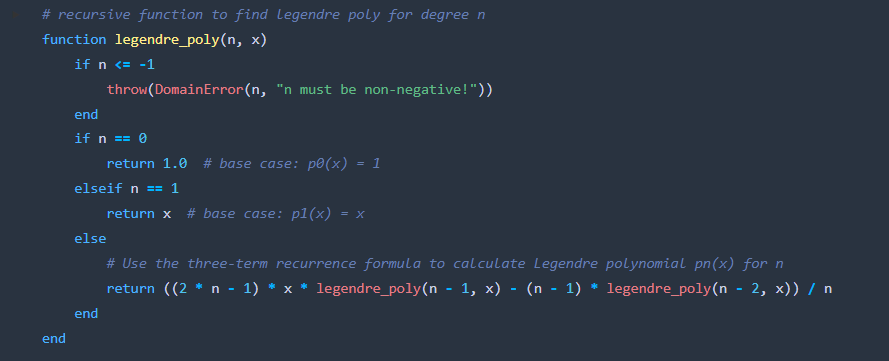
\includegraphics[scale=0.56]{leg-poly.png}
%\caption{three-term recurrence relation as julia function}
%\end{figure}

%\begin{figure}[ht]
%\centering
%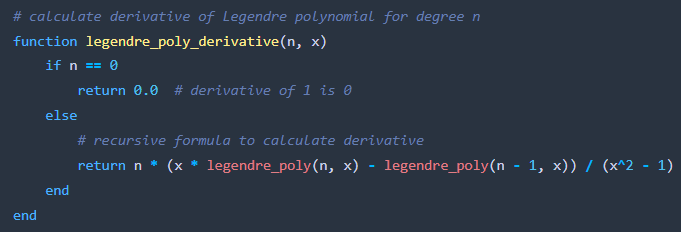
\includegraphics[scale=0.75]{deriv.png}
%\caption{\(P'_n(x)\) as julia function}
%\end{figure}

Now  I can calculate the roots and weights for each Legendre polynomial. The primary function computes the roots and weights of the Legendre polynomials based on the given degree n. To find the roots of each polynomial, I call my \textit{legendre\_poly()} function with the necessary values then essentially set \(P_n(x_i) = 0\). In Julia, you can utilize the \textbf{Roots.jl} package and call the \textit{findzeros()} function. From there the weights are found using the two formulas above.

\textit{https://juliapackages.com/p/roots}

\begin{figure}[ht]
\centering
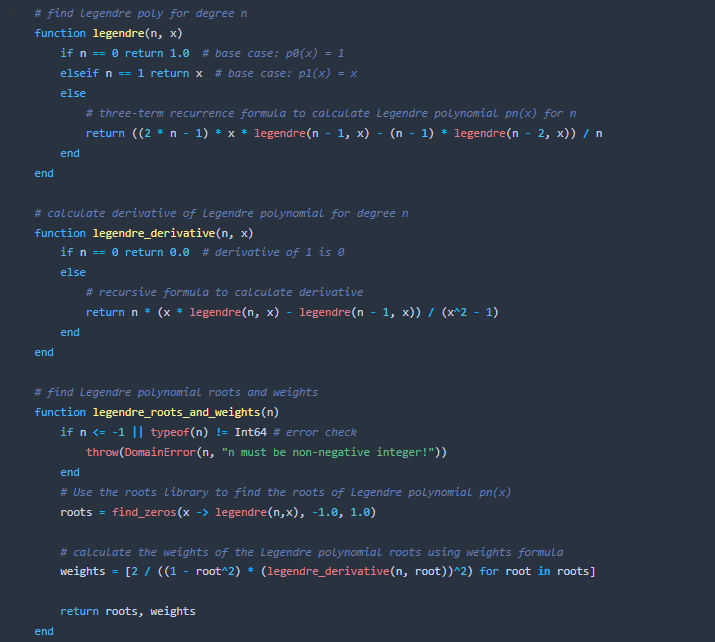
\includegraphics[scale=0.85]{img/functions.png}
\caption{Julia functions for computing Gauss-Legendre roots and weights}
\end{figure}

\newpage

%Now to visualize the data I run the following code


%\begin{figure}[ht]
%   \centering
%   \begin{minipage}{0.4\textwidth}
%        \centering
%        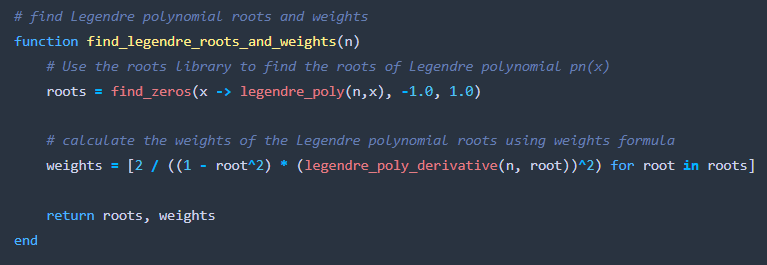
\includegraphics[scale=0.36]{roots-weights.png}
 %       \caption{find roots and weights}
%    \end{minipage}\hfill
%    \begin{minipage}{0.55\textwidth}
%        \centering
 %       \includegraphics[scale=0.42]{create-table.png}
 %       \caption{produce table of roots and weights per degree n}
 %   \end{minipage}
%\end{figure}

\section{Unit Testing}
Before code execution, it's important to conduct tests to verify all functions work. I start with importing the \textbf{FastGaussQuadrature.jl} and \textbf{LegendrePolynomials.jl} external packages, as well as the \textbf{Linear Algebra} and \textbf{Test} libraries. These external packages and libraries have been throughly tested and assist me in identifing potential flaws within my code. Note I don't cover all test cases, but these should be sufficient for what I'm trying to acheive. Refer to my code and comments for further details.

\textit{https://juliapackages.com/p/fastgaussquadrature} :  \textit{https://juliapackages.com/p/legendrepolynomials}\\
\textit{https://docs.julialang.org/en/v1/stdlib/LinearAlgebra/} : \textit{https://docs.julialang.org/en/v1/stdlib/Test/}


\begin{figure}[ht]
\centering
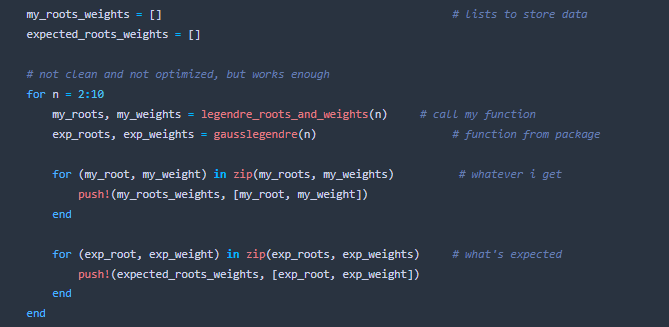
\includegraphics[scale=0.6]{img/store-all-data.png}
\caption{Storing my function and external gauss function in lists for unit tests}
\end{figure}

\begin{figure}[H]
\centering
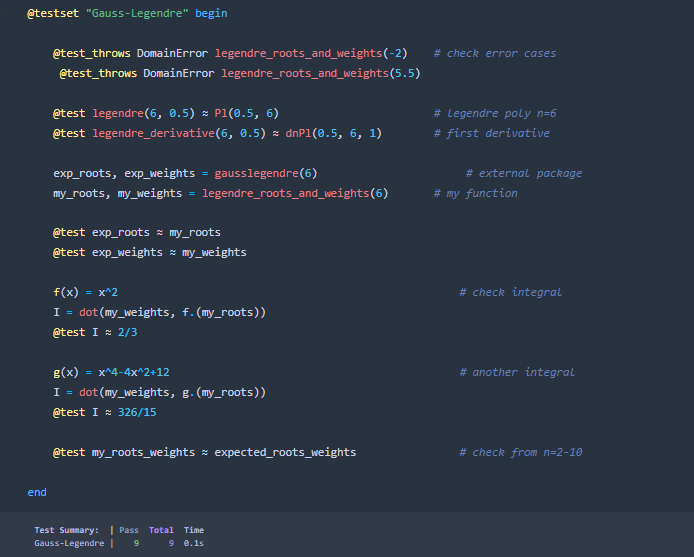
\includegraphics[scale=0.65]{img/test.png}
\caption{Unit tests}
\end{figure}

\newpage

\section{Results}

After executing the main code and utilizing the \textbf{PrettyTables.jl} package for data visualization, I have successfully obtained the roots and weights for each degree $n = 2, \ldots, 10$. The output table below presents the results. Refer to the next page to view the table more clearly.

\textit{https://juliapackages.com/p/prettytables}

\begin{figure}[ht]
\centering
\includegraphics[scale=0.75]{img/create-table.png}
\caption{Code to produce table of roots and weights of LP per degree n}
\end{figure}

\begin{figure}[H]
    \centering
    \begin{minipage}{0.5\textwidth}
        \centering
        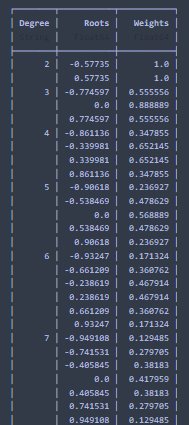
\includegraphics[scale=0.65]{img/table_2-7.png}
      %  \caption{Output table for degrees n = 2, ... , 7}
    \end{minipage}\hfill
    \begin{minipage}{0.5\textwidth}
        \centering
        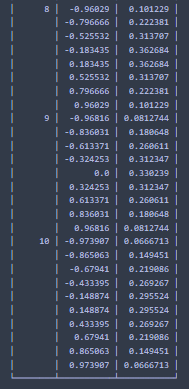
\includegraphics[scale=0.65]{img/table_8-10.png}
        %\caption{Output table for degrees n = 8, 9, 10}
    \end{minipage}
\caption{Julia output table of roots and weights of LP degrees n = 2, ... , 10}
\end{figure}



\newpage

\begin{table}[H]
\centering
\scalebox{0.95} {
\begin{tabular}{|c|c|c|}
\hline
Degree n & Roots \(x_i\) & Weights \(w_i\) \\
\hline
2 & -0.57735 & 1.0 \\
 & 0.57735 & 1.0 \\
\hline
3 & -0.774597 & 0.555556 \\
 & 0.0 & 0.888889 \\
 & 0.774597 & 0.555556 \\
\hline
4 & -0.861136 & 0.347855 \\
 & -0.339981 & 0.652145 \\
 & 0.339981 & 0.652145 \\
 & 0.861136 & 0.347855 \\
\hline
5 & -0.90618 & 0.236927 \\
 & -0.538469 & 0.478629 \\
 & 0.0 & 0.568889 \\
 & 0.538469 & 0.478629 \\
 & 0.90618 & 0.236927 \\
\hline
6 & -0.93247 & 0.171324 \\
 & -0.661209 & 0.360762 \\
 & -0.238619 & 0.467914 \\
 & 0.238619 & 0.467914 \\
 & 0.661209 & 0.360762 \\
 & 0.93247 & 0.171324 \\
\hline
7 & -0.949108 & 0.129485 \\
 & -0.741531 & 0.279705 \\
 & -0.405845 & 0.38183 \\
 & 0.0 & 0.417959 \\
 & 0.405845 & 0.38183 \\
 & 0.741531 & 0.279705 \\
 & 0.949108 & 0.129485 \\
\hline
8 & -0.96029 & 0.101229 \\
 & -0.796666 & 0.222381 \\
 & -0.525532 & 0.313707 \\
 & -0.183435 & 0.362684 \\
 & 0.183435 & 0.362684 \\
 & 0.525532 & 0.313707 \\
 & 0.796666 & 0.222381 \\
 & 0.96029 & 0.101229 \\
\hline
9 & -0.96816 & 0.0812744 \\
 & -0.836031 & 0.180648 \\
 & -0.613371 & 0.260611 \\
 & -0.324253 & 0.312347 \\
 & 0.0 & 0.330239 \\
 & 0.324253 & 0.312347 \\
 & 0.613371 & 0.260611 \\
 & 0.836031 & 0.180648 \\
 & 0.96816 & 0.0812744 \\
\hline
10 & -0.973907 & 0.0666713 \\
 & -0.865063 & 0.149451 \\
 & -0.67941 & 0.219086 \\
 & -0.433395 & 0.269267 \\
 & -0.148874 & 0.295524 \\
 & 0.148874 & 0.295524 \\
 & 0.433395 & 0.269267 \\
 & 0.67941 & 0.219086 \\
 & 0.865063 & 0.149451 \\
 & 0.973907 & 0.0666713 \\
\hline
\end{tabular} 
}

\caption{Roots and Weights for LP of degrees n= 2, ... , 10}
\end{table}

\newpage

\section{Optimization}

Here you can see the computation time and memory allocation of my custom function and \textbf{FastGaussQuadrature.jl} gauss-legendre function for when n = 10.

%\begin{figure}[ht]
%\centering
%\includegraphics[scale=0.9]{timer.png}
%\caption{compare computation time of functions (n=10)}
%\end{figure}

%\begin{figure}[ht]
%\centering
%\includegraphics[scale=0.9]{time-n=25.png}
%\caption{compare computation time of functions (n=25)}
%\end{figure}

\begin{figure}[ht]
   \centering
   \begin{minipage}{0.45\textwidth}
        \centering
        \includegraphics[scale=0.65]{img/timer.png}
       \caption{Computation time for n=10}
    \end{minipage}\hfill
    \begin{minipage}{0.55\textwidth}
        \centering
        \includegraphics[scale=0.65]{img/time-n=25.png}
        \caption{Computation time for n=25}
    \end{minipage}
\end{figure}

Initially with n = 10, the difference is relatively insignificant. However when n = 25, the divergence in both computation time and memory allocation become more pronounced and is even bigger when n becomes larger. 
%Note that my function uses recursion, which significantly impacts performance when n becomes large.
Nonetheness, I only needed to find the results for degress \(n= 2, ... , 10\) so the recursive methods were simplest to implement and are sufficient.

Now what IF I want to use Gauss-Lengendre for \(n \ge 1000\)? My recursive methods are not efficient enough due to extra memory usage, and overhead of function calls and returns. % Optimizing the code for speed often involves improving algorithmic efficiency and reducing unnecessary computations. 
In my code, the most significant potential for optimization lies in caching and reusing intermediate results and avoiding repeated calculations. Two basic techniques to solve this are using memoization (top-down) or an iterative (bottom-up) approach.\(^{[7]}\) I won't go too in-depth, but here are some brief explanations. %Calculating the Fibonacci number is shown as an example.

%\subsubsection*{Memoization Approach}
\textbf{Memoization Approach:}
From [7], memoization caches and reuses prior results, specifically storing intermediate Legendre polynomial calculations for different \textit{n} values. This approach optimizes efficiency by eliminating redundant recursive function calls and efficiently retrieving precomputed Legendre polynomials.
%It's particularly advantageous when recalculating Legendre polynomials of the same degree, eliminating the need for redundant recomputation.
\begin{small}
\begin{verbatim}
# basic idea for memoization for legendre polys; can be applied to p'n(x)
memo = (use dictionary or hashmap) # cache poly calculations
function memo_legendre(n, x)
  if key=(n,x) in memo # reduces extra calculations
    return memo[key=(n,x)]
  if ... # base cases for n = 0 or 1
  else result = (three-term formula) # use recursion
  memo[key=(n,x)] = result # cache for future use
  return result
\end{verbatim}
\end{small}

%\subsubsection*{Iterative Approach}
\textbf{Iterative Approach:}
From [7], iteration employs loops and constructs to eliminate function call and recursion overhead. By initializing and updating variables within a loop, it creates efficient computation, minimizes memory usage, and prevents stack overflow issues.

\begin{small}
\begin{verbatim}
# basic idea for iterative approach for legendre polys; can be applied to p'n(x)
function iterative_legendre(n,x)
  if ... # base cases for n = 0 or 1
  else
    p0, p1 = 1, x # init first two legendre polys
    for i in 2:n
      p0, p1 = p1, (three-term formula) # update values
    end
    return p1
\end{verbatim}
\end{small}

%Both the memoization and iterative approaches are superior to pure recursion. However, when dealing with high-degree Legendre polynomials \(n \ge 1000\), the iterative approach outperforms in both time and space complexity.  If I were to rewrite the code, I would take the time and optimize using a bottom-up approach.

% By combining memoization and transitioning to an iterative approach, your code becomes more memory-efficient and significantly faster, particularly when dealing with high-degree Legendre polynomials. These optimizations effectively reduce redundant calculations and make your code more resilient and robust, ensuring it performs well even for the most demanding computational tasks.

%Memoization is a technique that involves caching and reusing previously computed results. In the context of Legendre polynomials, it means storing the results of intermediate Legendre polynomial calculations for specific degrees and values of 'x.'
%As 'n' becomes large, the number of recursive function calls and redundant calculations also grows. By employing memoization, you can efficiently store and retrieve previously computed Legendre polynomials, saving considerable computational time.
%This technique is particularly beneficial when calculating Legendre polynomials for the same degree multiple times, as it avoids the need to recompute these values from scratch.

%The transition from a recursive to an iterative approach is crucial when working with high-degree Legendre polynomials. This shift improves both computational efficiency and code robustness.
%Recursive methods can lead to stack overflow errors for extremely high degrees, whereas an iterative approach uses loops and iterative constructs to avoid the overhead of function calls and recursion.
%It involves initializing variables to store intermediate results, and then updating these variables within a loop to calculate Legendre polynomials efficiently. This approach simplifies the computation, reduces memory usage, and prevents stack overflow issues.

%The most obvious thing to modify is using iterative methods instead of recursion. The transition from a recursive to an iterative approach for higher degrees not only enhances efficiency but also prevents stack overflow issues, making our code more robust.

%Memoization: Use memoization to store and reuse previously calculated Legendre polynomials and their derivatives. This can significantly reduce redundant calculations, especially when %computing Legendre polynomials for the same degree multiple times.

%Optimize Weight Calculation: Since Legendre polynomial derivatives are already memoized, you can avoid recalculating the derivative inside the weight calculation loop. Compute the derivatives for all roots once and store them in an array.

%These optimizations should help reduce redundant calculations and make your code run faster, especially when calculating Legendre polynomials for larger degrees.

%Gauss-Legendre Quadrature is a formidable and efficient method for accurate numerical integration. This report has demonstrated the implementation of this technique in Julia, providing roots and weights for degrees  \(n= 2, ... , 10\). The principles discussed here are versatile and can be applied to address a wide array of numerical integration challenges across diverse scientific and engineering domains.

\newpage

\section{Conclusion}

I'll proceed with a quick application of my custom Gauss-Legendre functions to approximate

\[
%f(x) = \frac{1}{2}e^{-(\frac{1+x}{2})^2}
f(x) = e^x cos(x) \Longrightarrow \int_{-1}^{1} e^x cos(x) dx
\]

This integral is an example from B\&F 4.7\(^{[1]}\). I'll utilize the \textbf{QuadGK.jl} package to calculate a precise value and then compare it to the approximations I've generated. The outcomes are presented in code below.

\textit{https://juliamath.github.io/QuadGK.jl/stable/}

\begin{figure}[ht]
\centering
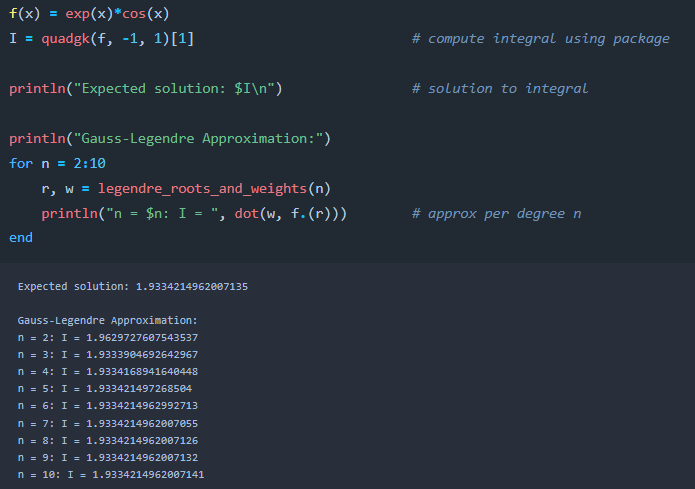
\includegraphics[scale=0.8]{img/apprx.png}
\caption{Approximations of definite integral from B\&F 4.7}
\end{figure}

For \(f(x)\), you can see a higher order rule generally gives a better approximation to the required integration. This continuous improvement in accuracy highlights the practical advantage of employing higher-order Gauss-Legendre quadrature rules.

In conclusion, Gauss-Legendre quadrature is a highly effective method for accurately approximating definite integrals within the interval \([-1, 1]\). This numerical integration technique strategically selects a set of roots and weights based on associated orthogonal Legendre polynomials, providing an efficient approach. Applications of Gauss-Legendre quadrature extends across various fields, including mathematics, physics, engineering, and other scientific disciplines. Its reliability in achieving high precision makes it a preferred choice for accurate numerical integration in various computational applications.
\newpage

%\(^{[1]}\)

\begin{thebibliography}{9}
\bibitem{BF}
Burden, R. L., \(\&\) Faires, J. D. (2015). Numerical Analysis (10th ed.) Sec 4.7, pg 229-232. Brooks/Cole (Cengage Learning).

\bibitem{wolf}
Wolfram Research. (2023, November). Legendre Polynomial. MathWorld.\\ URL: https://mathworld.wolfram.com/LegendrePolynomial.html

\bibitem{koepf}
Koepf, W. Hypergeometric Summation: An Algorithmic Approach to Summation and Special Function Identities, pg 2. Braunschweig, Germany: Vieweg, 1998.

\bibitem{libretext}
Herman, Russell. University of North Carolina Wilmington, LibreTexts. (2023, November). Legendre Polynomials. In A First Course in Differential Equations for Scientists and Engineers (Herman). \\ URL: https://math.libretexts.org/Bookshelves/Differential\_Equations/At\_First\_Course\_in\_Differential\_
Equations\_for\_Scientists\_and\_Engineers\_(Herman)/04\%3A\_Series\_Solutions/4.05\%3A\_Legendre\_Polynomials

\bibitem{hildebrand}
Hildebrand, F. B. Introduction to Numerical Analysis, pg 324. New York: McGraw-Hill, 1956.

\bibitem{weightform}
Abramowitz, Milton; Stegun, Irene Ann, eds. (1983) [June 1964]. "Chapter 25.4, Integration". Handbook of Mathematical Functions with Formulas, Graphs, and Mathematical Tables. Applied Mathematics Series. Vol. 55 (Ninth reprint with additional corrections of tenth original printing with corrections (December 1972); first ed.). Washington D.C.; New York: United States Department of Commerce, National Bureau of Standards; Dover Publications. ISBN 978-0-486-61272-0. LCCN 64-60036. MR 0167642. LCCN 65-12253.

\bibitem{DP}
BasuMallick,  Chiradeep. (2022, October 19) What is Dynamic Programming? SpiceWorks. \\ URL: https://www.spiceworks.com/tech/devops/articles/what-is-dynamic-programming/

\end{thebibliography}

Source code and jupyter notebook are available upon request.


%\section*{Modifications}

%Since the three-term recurrence relation is a recursive formula, it may run slower and cause a stack overflow for larger degrees. To combat this, I can modify the functions and use
%iterative methods. This will not only lower the memory needed, but allow the program to run faster.

%\begin{figure}[ht]
%\centering
%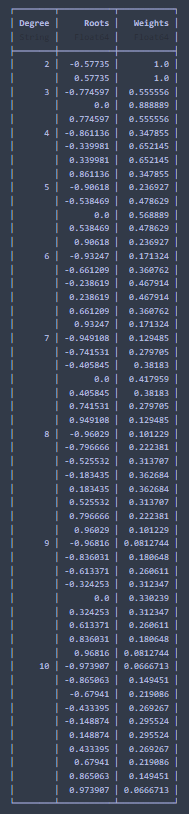
\includegraphics[scale=0.6]{output-table.png}
%\caption{function to produce table of roots and weights per degree n}
%\end{figure}


%\[ \frac{d}{dx} P_n(x) = \frac{d}{dx} \left[ \frac{1}{n} \left[ (2n-1) x P_{n-1}(x) - (n-1) P_{n-2}(x) \right] \right] \]


% **** THIS ENDS THE EXAMPLES. DON'T DELETE THE FOLLOWING LINE:

\end{document}





